% This file was created with tikzplotlib v0.9.17.
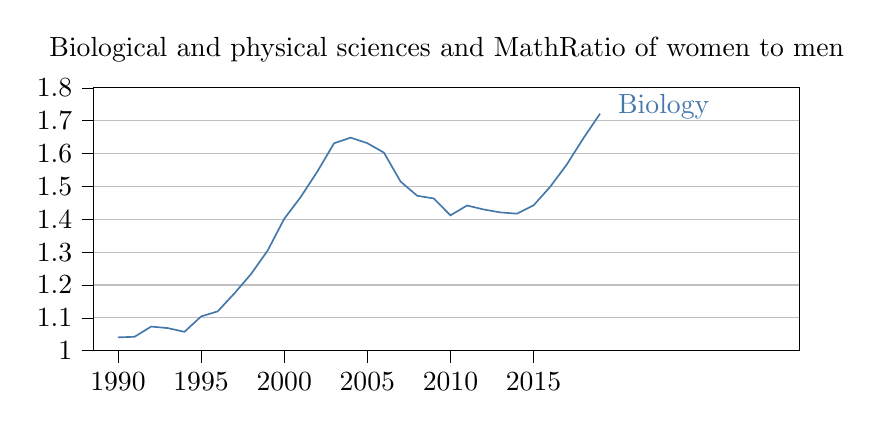
\begin{tikzpicture}

\definecolor{color0}{rgb}{0.266666666666667,0.466666666666667,0.666666666666667}

\begin{axis}[
height=140pt,
tick align=outside,
tick pos=left,
title={Biological and physical sciences and Math \\ Ratio of women to men},
width=300pt,
x grid style={white!69.0196078431373!black},
xmin=1988.55, xmax=2031,
xtick style={color=black},
xtick={1990,1995,2000,2005,2010,2015},
xticklabels={
  \(\displaystyle 1990\),
  \(\displaystyle 1995\),
  \(\displaystyle 2000\),
  \(\displaystyle 2005\),
  \(\displaystyle 2010\),
  \(\displaystyle 2015\)
},
ymajorgrids,
ymin=1, ymax=1.8,
ytick style={color=black},
ytick={1,1.1,1.2,1.3,1.4,1.5,1.6,1.7,1.8},
yticklabels={
  \(\displaystyle 1\),
  \(\displaystyle 1.1\),
  \(\displaystyle 1.2\),
  \(\displaystyle 1.3\),
  \(\displaystyle 1.4\),
  \(\displaystyle 1.5\),
  \(\displaystyle 1.6\),
  \(\displaystyle 1.7\),
  \(\displaystyle 1.8\)
}
]
\addplot [semithick, color0]
table {%
1990 1.04078304767609
1991 1.04256737232208
1992 1.07366561889648
1993 1.06894600391388
1994 1.05757308006287
1995 1.10440194606781
1996 1.11996006965637
1997 1.17428719997406
1998 1.23312425613403
1999 1.30454993247986
2000 1.40134906768799
2001 1.46844744682312
2002 1.54577028751373
2003 1.63139522075653
2004 1.64863216876984
2005 1.63168549537659
2006 1.602987408638
2007 1.51491057872772
2008 1.47168242931366
2009 1.46346211433411
2010 1.41208970546722
2011 1.44205784797668
2012 1.42999362945557
2013 1.42106962203979
2014 1.41722071170807
2015 1.44253933429718
2016 1.49894797801971
2017 1.56678104400635
2018 1.64683747291565
2019 1.72139155864716
};
\draw (axis cs:2019.5,1.72139153632667) node[
  anchor=base west,
  text=color0,
  rotate=0.0
]{Biology};
\end{axis}

\end{tikzpicture}

\vspace{0.1cm}
\begin{tikzpicture}
% This file was created with tikzplotlib v0.9.17.
\definecolor{color0}{rgb}{0.266666666666667,0.466666666666667,0.666666666666667}

\begin{groupplot}[group style={group size=2 by 1, horizontal sep=0.8cm, group name=my plots}]
\nextgroupplot[
height=90pt, width=160pt,
legend style={at={(2.02, 0.5)},anchor=west,},
reverse legend,
tick align=outside,
tick pos=left,
x grid style={white!69.0196078431373!black},
xlabel={Women},
xmin=1988.55, xmax=2020.45,
xtick style={color=black},
xtick={1990,2000,2010},
xticklabels={\(\displaystyle 1990\),\(\displaystyle 2000\),\(\displaystyle 2010\)},
ymajorgrids,
ymin=0, ymax=84.0126,
ytick style={color=black}
]
\path [draw=color0, fill=color0]
(axis cs:1990,19.14)
--(axis cs:1990,0)
--(axis cs:1991,0)
--(axis cs:1992,0)
--(axis cs:1993,0)
--(axis cs:1994,0)
--(axis cs:1995,0)
--(axis cs:1996,0)
--(axis cs:1997,0)
--(axis cs:1998,0)
--(axis cs:1999,0)
--(axis cs:2000,0)
--(axis cs:2001,0)
--(axis cs:2002,0)
--(axis cs:2003,0)
--(axis cs:2004,0)
--(axis cs:2005,0)
--(axis cs:2006,0)
--(axis cs:2007,0)
--(axis cs:2008,0)
--(axis cs:2009,0)
--(axis cs:2010,0)
--(axis cs:2011,0)
--(axis cs:2012,0)
--(axis cs:2013,0)
--(axis cs:2014,0)
--(axis cs:2015,0)
--(axis cs:2016,0)
--(axis cs:2017,0)
--(axis cs:2018,0)
--(axis cs:2019,0)
--(axis cs:2019,80.012)
--(axis cs:2019,80.012)
--(axis cs:2018,77.044)
--(axis cs:2017,74.455)
--(axis cs:2016,71.245)
--(axis cs:2015,67.896)
--(axis cs:2014,64.159)
--(axis cs:2013,61.484)
--(axis cs:2012,58.89)
--(axis cs:2011,55.388)
--(axis cs:2010,52.654)
--(axis cs:2009,51.148)
--(axis cs:2008,49.45)
--(axis cs:2007,48.209)
--(axis cs:2006,45.395)
--(axis cs:2005,42.742)
--(axis cs:2004,40.68)
--(axis cs:2003,39.731)
--(axis cs:2002,37.825)
--(axis cs:2001,37.162)
--(axis cs:2000,37.189)
--(axis cs:1999,37.331)
--(axis cs:1998,36.773)
--(axis cs:1997,34.928)
--(axis cs:1996,32.583)
--(axis cs:1995,29.63)
--(axis cs:1994,26.617)
--(axis cs:1993,24.543)
--(axis cs:1992,22.489)
--(axis cs:1991,20.304)
--(axis cs:1990,19.14)
--cycle;

\addplot [semithick, color0]
table {%
1990 19.1399993896484
1991 20.3040008544922
1992 22.4890003204346
1993 24.5429992675781
1994 26.617000579834
1995 29.6299991607666
1996 32.5830001831055
1997 34.9280014038086
1998 36.7729988098145
1999 37.3310012817383
2000 37.1889991760254
2001 37.1619987487793
2002 37.8250007629395
2003 39.7309989929199
2004 40.6800003051758
2005 42.742000579834
2006 45.3950004577637
2007 48.2089996337891
2008 49.4500007629395
2009 51.1479988098145
2010 52.6539993286133
2011 55.3880004882812
2012 58.8899993896484
2013 61.484001159668
2014 64.1589965820312
2015 67.8960037231445
2016 71.245002746582
2017 74.4550018310547
2018 77.0439987182617
2019 80.0120010375977
};

\nextgroupplot[
height=90pt, width=160pt,
legend style={at={(2.02, 0.5)},anchor=west,},
reverse legend,
tick align=outside,
tick pos=left,
x grid style={white!69.0196078431373!black},
xlabel={Men},
xmin=1988.55, xmax=2020.45,
xtick style={color=black},
xtick={1990,2000,2010},
xticklabels={\(\displaystyle 1990\),\(\displaystyle 2000\),\(\displaystyle 2010\)},
ymajorgrids,
ymin=0, ymax=49.9065,
ytick style={color=black}
]
\path [draw=color0, fill=color0]
(axis cs:1990,18.39)
--(axis cs:1990,0)
--(axis cs:1991,0)
--(axis cs:1992,0)
--(axis cs:1993,0)
--(axis cs:1994,0)
--(axis cs:1995,0)
--(axis cs:1996,0)
--(axis cs:1997,0)
--(axis cs:1998,0)
--(axis cs:1999,0)
--(axis cs:2000,0)
--(axis cs:2001,0)
--(axis cs:2002,0)
--(axis cs:2003,0)
--(axis cs:2004,0)
--(axis cs:2005,0)
--(axis cs:2006,0)
--(axis cs:2007,0)
--(axis cs:2008,0)
--(axis cs:2009,0)
--(axis cs:2010,0)
--(axis cs:2011,0)
--(axis cs:2012,0)
--(axis cs:2013,0)
--(axis cs:2014,0)
--(axis cs:2015,0)
--(axis cs:2016,0)
--(axis cs:2017,0)
--(axis cs:2018,0)
--(axis cs:2019,0)
--(axis cs:2019,46.481)
--(axis cs:2019,46.481)
--(axis cs:2018,46.783)
--(axis cs:2017,47.521)
--(axis cs:2016,47.53)
--(axis cs:2015,47.067)
--(axis cs:2014,45.271)
--(axis cs:2013,43.266)
--(axis cs:2012,41.182)
--(axis cs:2011,38.409)
--(axis cs:2010,37.288)
--(axis cs:2009,34.95)
--(axis cs:2008,33.601)
--(axis cs:2007,31.823)
--(axis cs:2006,28.319)
--(axis cs:2005,26.195)
--(axis cs:2004,24.675)
--(axis cs:2003,24.354)
--(axis cs:2002,24.47)
--(axis cs:2001,25.307)
--(axis cs:2000,26.538)
--(axis cs:1999,28.616)
--(axis cs:1998,29.821)
--(axis cs:1997,29.744)
--(axis cs:1996,29.093)
--(axis cs:1995,26.829)
--(axis cs:1994,25.168)
--(axis cs:1993,22.96)
--(axis cs:1992,20.946)
--(axis cs:1991,19.475)
--(axis cs:1990,18.39)
--cycle;

\addplot [semithick, color0]
table {%
1990 18.3899993896484
1991 19.4750003814697
1992 20.9459991455078
1993 22.9599990844727
1994 25.1679992675781
1995 26.8290004730225
1996 29.0930004119873
1997 29.7439994812012
1998 29.8209991455078
1999 28.6159992218018
2000 26.5380001068115
2001 25.306999206543
2002 24.4699993133545
2003 24.3540000915527
2004 24.6749992370605
2005 26.1949996948242
2006 28.3190002441406
2007 31.8229999542236
2008 33.601001739502
2009 34.9500007629395
2010 37.2879981994629
2011 38.4090003967285
2012 41.181999206543
2013 43.265998840332
2014 45.2709999084473
2015 47.0670013427734
2016 47.5299987792969
2017 47.5209999084473
2018 46.7830009460449
2019 46.4809989929199
};
\end{groupplot}




\end{tikzpicture}
\caption{Number Bachelor's degrees awarded (thousands). Source: IPEDS.}
